Web Browser haben sich seit der Veröffentlichung von Mosaic, einer der ersten populären Browser, im Jahr 1993 stark weiterentwickelt. Das Abrufen und Anzeigen von statischen HTML-Dokumenten wurde mit Hilfe von JavaScript um interaktive und später dynamische Inhalte erweitert. Heutzutage können in Browsern komplexe Webapplikationen realisiert werden, welche zudem unabhängig von einem speziellen Browser entwickelt werden können. Durch diese Entwicklung und die breiten Anwendungsfälle, besitzt die Umgebung \enquote{Browser} besondere Eigenschaften, welche nachfolgend beschrieben werden.

\subsection{Browserprodukte}
\label{sec:browserprodukte}

\begin{wrapfigure}[19]{r}{0.45\textwidth}
\centering
\tikzsetnextfilename{cross-browser_metastudie}
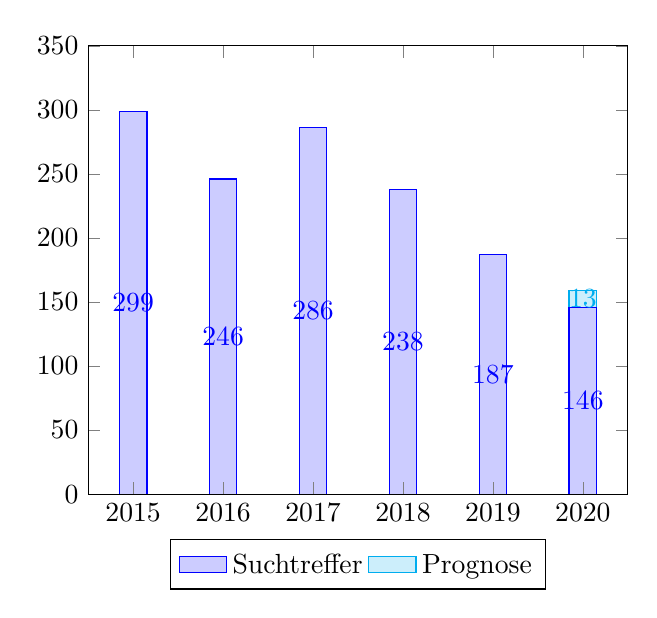
\begin{tikzpicture}
	\begin{axis}[
		ybar stacked,
        ymin=0,
        ymax=350,
        ytick distance={50},
		area style,
		legend style={at={(0.5,-0.10)},anchor=north,legend columns=-1},
		nodes near coords,
		symbolic x coords = {2015, 2016, 2017, 2018, 2019, 2020},
	]
		\addplot+[blue,fill opacity=0.2,text opacity=1,ybar,no marks]
			plot coordinates {
			(2015,299)
			(2016,246)
			(2017,286)
			(2018,238)
			(2019,187)
			(2020,146)
			};
		\addplot+[cyan,fill opacity=0.2,text opacity=1,ybar,no marks]
			plot coordinates {
			(2015,0)
			(2016,0)
			(2017,0)
			(2018,0)
			(2019,0)
			(2020,13)
			};
		\legend{\strut Suchtreffer, \strut Prognose}
	\end{axis}
\end{tikzpicture}
\caption{Studien zur Browserkompatibilität, eigene Darstellung (vgl. \ref{sec:studien-zur-browser-kompatibilitaet})}
\label{fig:studien-zur-browser-kompatibilitaet}
\end{wrapfigure}

Die Vielfalt an Browsern bereitet Webentwicklern immer wieder eine Herausforderung, dass ein von ihnen bereitgestelltes Produkt für die Nutzer einwandfrei funktioniert, unabhängig ihrer Browserpräferenz. Die Häufigkeit solcher Probleme, auch Cross-Browser-Incompatibilities (XBI) genannt, hat jedoch abgenommen, unter anderem erklärbar durch den Trend von offenen Web-Standards \cite{W3CStandards}.

Generell lässt sich feststellen, dass auch in der Literatur die Veröffentlichungen in Bezug auf (In-)Kompatibilität von Browsern abnimmt, dies ist in \autoref{fig:studien-zur-browser-kompatibilitaet} zu betrachten. Dies spricht dafür, dass das Problem von XBIs nicht mehr so präsent ist, wie zuvor.

Im Jahr 2020 gab es weitere Entwicklungen, die die Kompatibilität zwischen Browsern erhöhte. Microsoft ist beim Folgeprodukt zum Internet Explorer, den Microsoft Edge Browser, von einer proprietären Browserengine zu Chromium gewechselt \cite{MicrosoftEdgeChromium} und enthält somit denselben Kern wie Chrome und Opera. Zum Ende 2020 wird zudem der Support für den Internet Explorer 11 eingestellt \cite{MicrosoftInternetExplorerDeprecation}. Im September 2020 meldete Statista eine Marktverteilung von 69,71\% Chrome, 8,73\% Safari, 8,15\% Firefox, 5,54\% Edge, 2,51\% Internet Explorer und 2,3\% Opera \cite{StatistaBrowserMarketshare}.

\subsection{JavaScript}

Als JavaScript 1997 veröffentlicht und in den NetScape Navigator integriert wurde, gab es die berechtigen Bedenken, dass das Öffnen einer Webseite dem Betreiber erlaubt Code auf dem System eines Nutzers auszuführen. Damit dies nicht eintritt, wurde der JavaScript Ausführungskontext in eine virtuelle Umgebung integriert, einer Sandbox. \cite{LearningJavaScript}

Die JavaScript-Sandbox bei Browsern schränkt ein, dass unter anderem kein Zugriff auf das Dateisystem erfolgen kann. Auch Zugriff auf native Bibliotheken oder Ausführung von nativem Code ist nicht möglich \cite{TheSpyInTheSandbox}. Browser bieten dafür aber einige Schnittstellen an, die es erlauben z. B. Daten beim Client zu speichern oder auch Videos abzuspielen.

\nomenclature[Fachbegriff]{CORS}{Cross-Origin Resource Sharing}
\nomenclature[Fachbegriff]{Ajax}{Asynchronous JavaScript and XML}
\nomenclature[Fachbegriff]{W3C}{World Wide Web Consortium}
\nomenclature[Fachbegriff]{XHR}{XMLHttpRequest}

Microsoft nahm 1999 im Internet Explorer 5.0 eine neue Methode in ihre JavaScript-Umgebung auf: Ajax (Asynchronous JavaScript and XML). Ajax erlaubt die Datenabfrage von Webservern mittels JavaScript. Hierdurch wird ermöglicht, dass Inhalte auf Webseiten dynamisch abgefragt und dargestellt werden können, zuvor war hierfür ein erneuter Seitenaufruf notwendig. Das Konzept wurde kurz darauf von allen damals gängigen Browser übernommen. Erst jedoch mit der Standardisierung 2006 durch das W3C \cite{TheXMLHttpRequestObject} fand die Methode Anklang und Einsatz bei Entwicklern und ist seitdem der Grundstein für unser dynamisches und interaktives Web \cite{TheStoryOfXMLHTTP}.

Webapplikationen wurden nun immer beliebter, aber Entwickler klagten darüber, dass Browser die Abfragen von JavaScript nur auf dem bereitstellenden Webserver, also \enquote{same-origin}, erlauben\cite{CrossSiteXHRWithCORS}. Im selben Jahr der Standardisierung von Ajax, wurde ein erster Entwurf zur Ermöglichung und Absicherung von Abrufen domänenfremder Ressourcen eingereicht \cite{AuthorizingCORS}, das sogenannte Cross-Origin Resource Sharing.

Über die Jahre wurde der JavaScript Standard immer umfangreicher und dies erlaubte Entwicklern mächtige Werkzeuge sowie Frameworks zu entwickeln, um u. A. Webapplikationen bereitzustellen. Webapplikationen konnten nun dazu verwendet werden, um einen großen Teil der Funktionalitäten eines Produktes abzubilden. Diese \enquote{clientbasierten} Anwendungen werden im nächsten Abschnitt näher beleuchtet.

% Im folgenden Abschnitt werden, für diese Arbeit relevante, Sicherheitsvorkehrungen von Browsern vorgestellt und beschrieben - darunter auch Cross-Origin Resource Sharing.

%\subsubsection{Fehleranfälligkeit}
%
%Die Sprache JavaScript stellt an sich auch eine Besonderheit der Umgebung dar. Denn anders als z. B. C, C++, Java gilt sie als fehleranfällig \cite{FastReproducingWebApplicationErrors}. Dies
